\documentclass[12pt, fullpage,letterpaper]{article}

\usepackage[margin=1in]{geometry}
\usepackage{graphicx}
\usepackage{amsmath,amssymb,graphicx,bbm}
\usepackage{amsthm,verbatim}
\usepackage{mathrsfs,mathtools}
\usepackage{float}

\usepackage[footnotesize,bf]{caption}
% \usepackage[left=1.1in,right=1.1in,top=1in]{geometry}

\newcommand{\bs}[1]{\boldsymbol{#1}}
\newcommand{\mathd}{\textrm{d}}
\newcommand{\ddx}[1]{\frac{\mathd}{\mathd #1}}
\newcommand{\N}{\mathbbm{N}}
\newcommand{\R}{\mathbbm{R}}

%% Patch for amsart date
\usepackage{etoolbox}
\makeatletter
\patchcmd{\@maketitle}
  {\ifx\@empty\@dedicatory}
  {\ifx\@empty\@date \else {\vskip3ex \centering\footnotesize\@date\par\vskip1ex}\fi
   \ifx\@empty\@dedicatory}
  {}{}
\patchcmd{\@adminfootnotes}
  {\ifx\@empty\@date\else \@footnotetext{\@setdate}\fi}
  {}{}{}
\makeatother
%%

\usepackage[dvipsnames]{xcolor}
\newcommand{\an}[1]{{\leavevmode\color{BrickRed}{#1}}}

\title{Project 1: Finite difference methods}
\author{Anka Chen}
\date{\today}

\begin{document}
\maketitle

\an{You should really keep the problem statement in here; otherwise you will forget what this report is talking about if you read it later.}

\section{Finite difference methods in 1D}
\subsection{Local Truncation Error}
First let's write out the $\widetilde{D}_0 \left( \kappa(x_j) \widetilde{D}_0 u_j \right)$ operator explicitly:
\begin{equation}
\begin{split}
    \widetilde{D}_0 \left( \kappa(x) \widetilde{D}_0 u(x)) \right) &= \widetilde{D}_0 \left(\kappa(x) \frac{u(x+h/2) - u(x-h/2}{h} \right)\\
    &= \kappa(x+h/2)\frac{u(x+h) - u(x)}{h^2} - \kappa(x-h/2)\frac{u(x) - u(x-h)}{h^2} \\
\end{split}
\end{equation}
We do the Taylor expansion for $\kappa$ at the point $x$:
\begin{equation}
  \kappa(x+h/2)=\an{\kappa}(x) + \kappa'(x)\frac{h}{1} + \kappa''(x)\frac{h^2}{8}  + \kappa^{(3)}(x)\frac{h^3}{48} + o(h^3)
\end{equation}
similarly:
\begin{equation}
  \kappa(x-h/2)=\an{\kappa}(x) - \kappa'(x)\frac{h}{1} + \kappa''(x)\frac{h^2}{8}  - \kappa^{(3)}(x)\frac{h^3}{48} + o(h^3)
\end{equation}

We do Taylor expansion for $u$ at the point $x$ as well: 
\begin{equation}
u(x+h) - u(x)= u'(x)h + u''(x)\frac{h^2}{2} + u^{(3)}\frac{h^3}{6} + u^{(4)}(x)\frac{h^4}{24} + o(h^4)
\end{equation}
\begin{equation}
u(x) - u(x-h)= u'(x)h - u''(x)\frac{h^2}{2} + u^{(3)}\frac{h^3}{6} - u^{(4)}(x)\frac{h^4}{24} + o(h^4)
\end{equation}

Then we can have the expansion of $\widetilde{D}_0 \left( \kappa(x) \widetilde{D}_0 u(x))\right)$:
\begin{equation}
\begin{split}
\widetilde{D}_0 \left( \kappa(x) \widetilde{D}_0 u(x))\right) &= \kappa(x)\left[ u''(x)+u^{(4)}\frac{h^2}{12} +o(h^2) \right]\\
&+\frac{h}{2}\kappa'(x) \left[\frac{2u'(x)}{h} + \frac{u^{(3)}(x)h}{3} + o(h)\right]\\
&+\frac{h^2}{8}\kappa'(x) \left[u''(x) + o(1)\right]\\
&= \kappa(x)u''(x) + \kappa'(x)u'(x) + \left[ \frac{\kappa(x)u^{(4)}(x)}{12} + \frac{\kappa'(x)u^{(3)}(x)}{6} + \frac{\kappa''(x)u''(x)}{8}\right]h^2 +o(h^2)
\end{split}
\end{equation}
Since $\ddx{x} \left(\kappa(x) \ddx{x} u(x) \right) = \kappa(x)u''(x) + \kappa'(x)u'(x)$, the local truncation error is:
\begin{equation}
\begin{split}
\text{LTE} = \widetilde{D}_0 \left( \kappa(x) \widetilde{D}_0 u(x))\right) - \ddx{x} \left(\kappa(x) \ddx{x} u(x) \right) \\
=  \left[ \frac{\kappa(x)u^{(4)}(x)}{12} + \frac{\kappa'(x)u^{(3)}(x)}{6} + \frac{\kappa''(x)u''(x)}{8}\right]h^2 +o(h^2)
\end{split}
\end{equation}
Thus this is a second-order scheme.

\subsection{Local Truncation Error}
\an{Did you mean to title this section something different?}
Denote $\kappa(x_j-h/2)$ as $k_{j-1/2}$ and  $\kappa(x_j+h/2)$ as $k_{j+1/2}$, we can convert the operator to a matrix:
\begin{equation}
\mathbf{A}=
\begin{bmatrix}
-k_{1+1/2}-k_{1-1/2} & k_{1+1/2} &0 & \hdots & 0 \\
k_{2-1/2} & - k_{2+1/2}-k_{2-1/2} & k_{2+1/2} &\hdots & 0 \\
\vdots &  \vdots  & \ddots & \vdots \\
0 & 0 & 0 & k_{M-1/2} & -k_{M+1/2}-k_{M-1/2} 
\end{bmatrix}  \frac{1}{h^2}
\end{equation}

I pick $u(x)=sin(\pi x), x \in [0,2]$ as the input function, see Fig. \ref{fig:solution}a.
I compute $f$ analytically:
\begin{equation}
  f(x) = \an{\kappa}'(x)u'(x) + \an{\kappa}(x)u''(x)
\end{equation}
I also confirmed the approximation of $f$ given by $\vec{f}_{approx} = A \vec{u}$, to make sure it is correct, see  Fig. \ref{fig:solution}bc.

\begin{figure}[H]
    \centering
    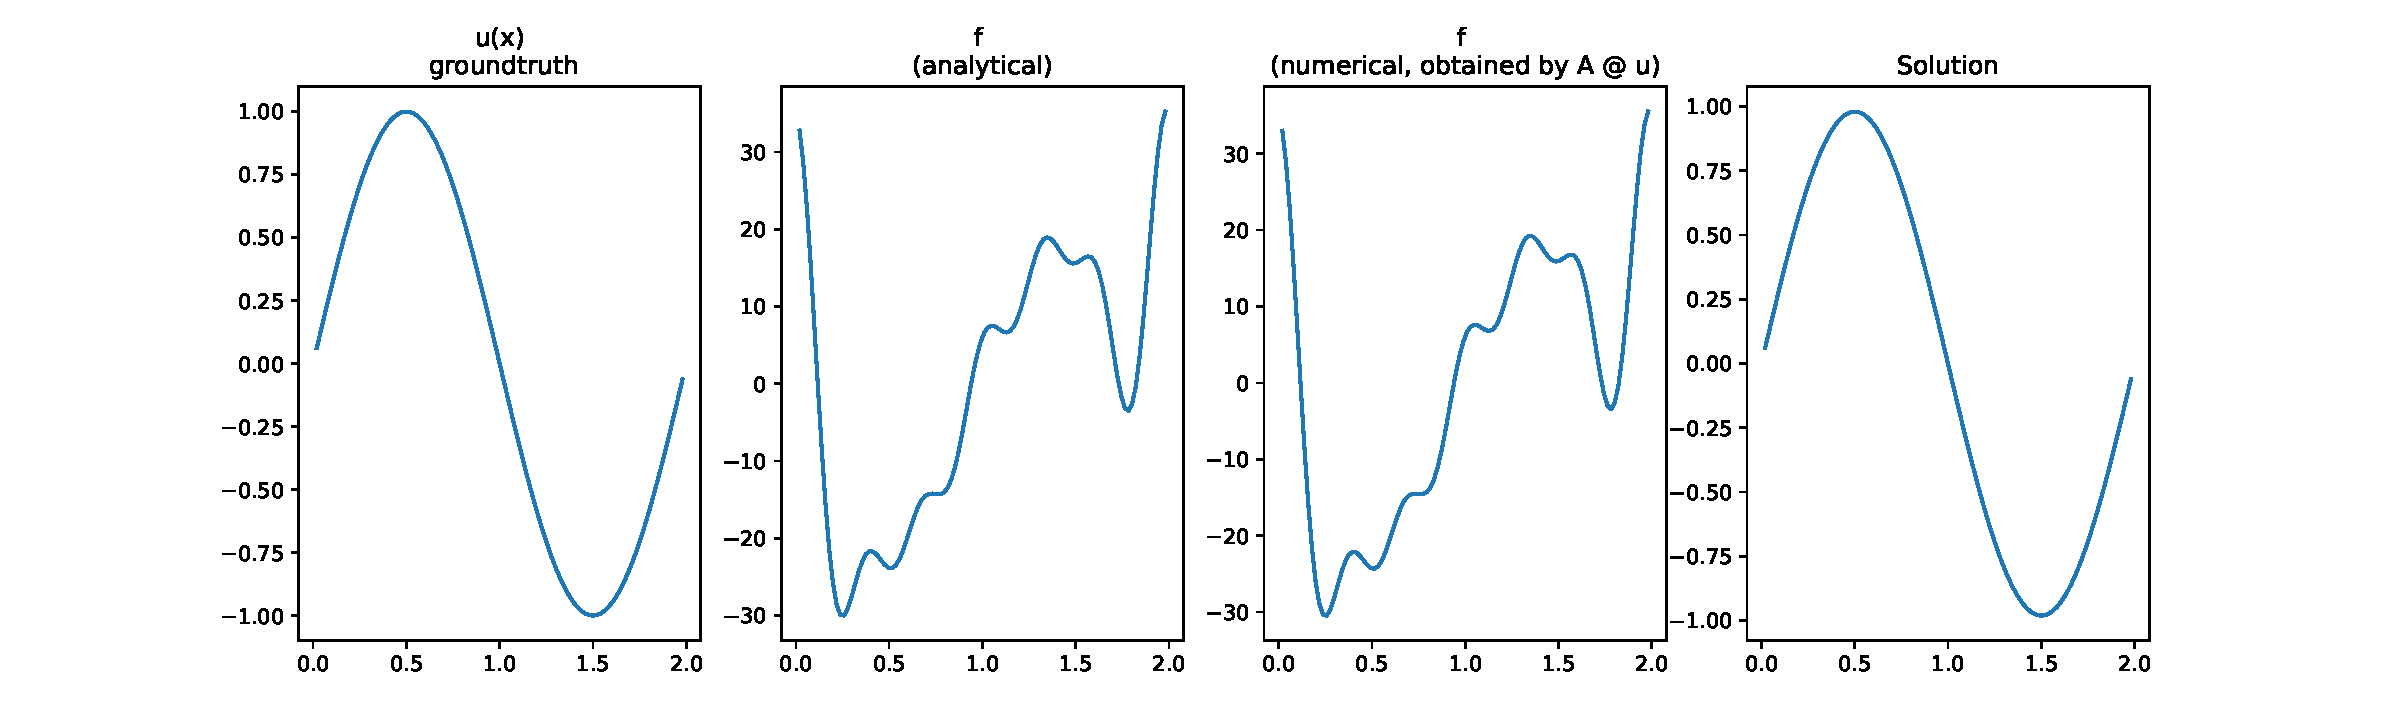
\includegraphics[width=1\textwidth]{Problem1/solution.pdf}
    \caption{Results generated from my solution programming: (a) the input $u(x)$, (b) the analytical $f$ computed by differentiating $u(x)$, (c) the numerical approximation of $f$, and (d) the solution of the ODE given by solving the linear system. }
    \label{fig:solution}
\end{figure}
\subsection{Solving}
Please see Fig.\ref{fig:error} for how the error and LTEs related to the steps of discretization. Both of those curves have a slope of -2.
\begin{figure}[H]
    \centering
    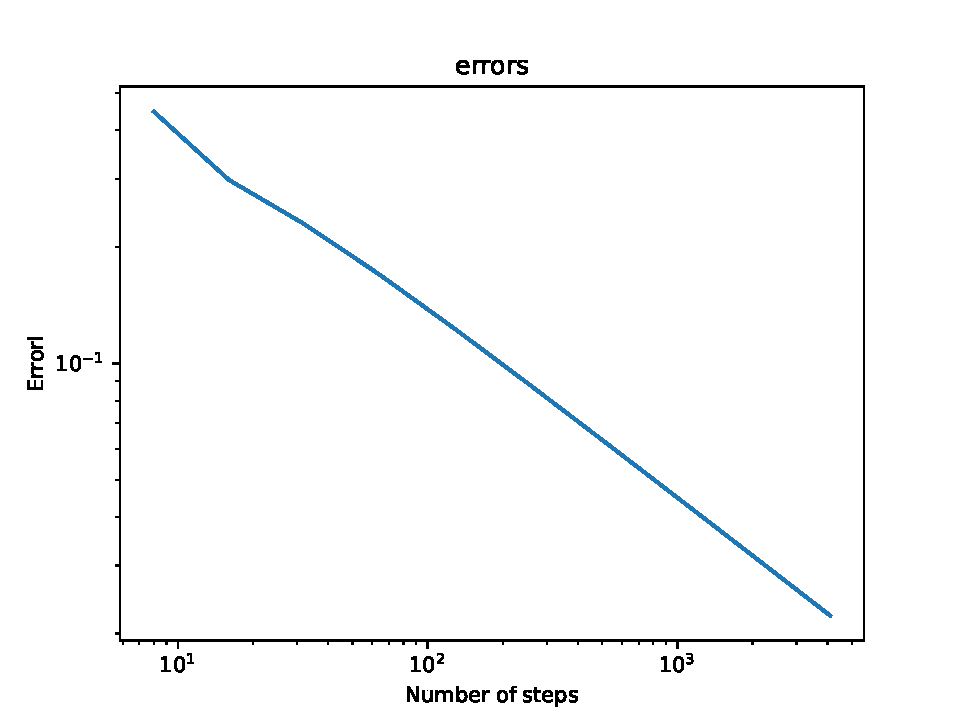
\includegraphics[width=0.6\textwidth]{Problem1/Error.pdf}
    \caption{How the errors and the LTEs changes with the steps of discretization. }
    \label{fig:error}
\end{figure}

\paragraph{An interesting finding}: When I am implementing the algorithm, I mistakenly computed $h$ as $\frac{1}{M+2}$ instead of  $\frac{1}{M+1}$. This will only affect the elements in $\mathbf{A}$. It turns out, even in this case, the solution will still converge, but with first-order accuracy. Because $h$ is computed incorrectly, it adds a first-order error term to the solution, making it a first-order scheme. 
\an{Yep, this is because
\begin{align*}
  \frac{1}{M+2} = \frac{1}{M+1} \left( 1 - \frac{1}{M+2}\right) \sim h \left(1 - h\right)
\end{align*}
i.e., replacing $M+1$ with $M+2$ causes relative error in $h$ of $\mathcal{O}(h)$, so that anything you compute makes an error of $\mathcal{O}(h)$.
}

\section{Finite difference methods in 2/3D }
\subsection{Discretization}
We just need to discretize the operator in two directions as we do in Problem 1:
\begin{equation}\label{eq:u2d}
\begin{split}
u_{xx}(x_i, y_i) = \frac{1}{h^2} \left[ { k_{i-1/2}u(x_{i-1}, y_i)  - (k_{i+1/2}-k_{i-1/2})u(x_{i}, y_i) -  k_{i+1/2}u(x_{i+1}, y_i) } \right]\\
u_{yy}(x_i, y_i) = \frac{1}{h^2} \left[ {  k_{i-1/2}u(x_{i}, y_{i-1})  - (k_{i+1/2}-k_{i-1/2})u(x_{i}, y_i) -  k_{i+1/2}u(x_{i}, y_{i+1} } \right]
\end{split}
\end{equation}
Then we have:
\begin{equation}
\nabla \cdot \left(\kappa(\bs{x}) \nabla \bs{u}(\bs{x}) \right) = \left[ u_{xx}(x_i, y_i) + u_{yy}(x_i, y_i) \right]_{i, j}
\end{equation}
The stencil is:
\begin{equation}
\begin{bmatrix}
  &k_{i-1/2} &  \\
k_{2-1/2} & -2(k_{2+1/2}-k_{2-1/2}) & k_{2+1/2}  \\
  &   k_{2+1/2}  &  

\end{bmatrix}  \frac{1}{h^2}
\end{equation}
\an{I don't think I understand your notation above (and below): you need double indices on $k$/$\kappa$ to properly index which direction you're shifting. E.g., in \eqref{eq:u2d} your $k_{i - 1/2}$ should mean two different across the equations.}
Note that I the direction of $x, y$ is defined using the matrix coordinate system, where the origin is at the top left corner. 
We discretize $u$ in both x and y direction with $M$ steps, and flatten it in column-major order, this gives us a vector $\mathbf{u} \in \mathbb{R}^{M^2}$. Similarly, we can convert the $\nabla \cdot \left(\kappa(\bs{x}) \nabla \bs{u}(\bs{x}) \right)$ to a linear operator on  $\mathbf{u}$, and the $(i + jM)$-th row of $\mathbf{A}$, which corresponds to  $u_{i,j}$ is:
\begin{equation}
\begin{matrix}
 \frac{1}{h^2}k_{2-1/2} & \dots & \frac{1}{h^2} k_{i-1-1/2} & \frac{-2}{h^2}(k_{2+1/2}-k_{2-1/2})& \frac{1}{h^2}k_{2+1/2}               & \dots &  \frac{1}{h^2}k_{2+1/2} \\
 [i + M(j-1)]\text{-th} &       &   [i-1 + jM]\text{-th}    &   [i + jM]\text{-th}   &   [i+1 + jM]\text{-th}  &       &    [i + (j+1)M]\text{-th}   
\end{matrix} 
\end{equation}

\an{I'm not sure why you decided to keep this 2D discussion in here...it's incomplete (as well as the code).}

% Consider the ordinary differential equation:
% \begin{align}\label{eq:ode}
%   \ddx{x} \left(\kappa(x) \ddx{x} u(x) \right) &= f(x), & x &\in [0,1],
% \end{align}
% with homogeneous Dirichlet boundary conditions, $u(0) = u(1) = 0$ , and where scalar diffusion coefficient $\kappa$ is given by,
%   \begin{align*}
%     \kappa(x) &= 2 + \sum_{\ell=1}^{5} \frac{1}{\ell+1} \sin( \ell \pi x ).
%   \end{align*}
%   The goal of this exercise will be to numerically compute solutions to this problem. \\[8pt]
%   \begin{itemize}
%     \item[(a)] Define the operator,
%       \begin{align*}
%         \widetilde{D}_0 u(x_j) &= \frac{u(x_j + h/2) - u(x_j - h/2)}{h/2}, & h &= 1/(N+1), & x_j &\coloneqq j h,
%       \end{align*}
%       for a fixed number of points $N \in \N$. Then with $u_j$ the numerical solution approximating $u(x_j)$ for solving the $d=1$ version of \eqref{eq:ode}, consider the scheme,
%       \begin{align}\label{eq:D0-def}
%         \widetilde{D}_0 \left( \kappa(x_j) \widetilde{D}_0 u_j \right) &= f(x_j), & j \in [N].
%       \end{align}
%       Show that, for smooth $u$ and $\kappa$, this scheme has second-order local truncation error.
%     \item[(b)] Construct an exact solution via the \textit{mathed of manufactured solutions}: posit an exact (smooth) solution $u(x)$ (that satisfies the boundary conditions!) and, compute $f$ in \eqref{eq:ode} so that your posited solutions satifies \eqref{eq:ode}. 
%     \item[(c)] Implement the scheme above for solving \eqref{eq:ode}, setting $f$ to be the function identified in part (b), so that you know the exact solution. Show that indeed you achieve second-order convergence in $h$ (say in the $h^{d/2}$-scaled vector $\ell^2$ norm) . (To ``show'' this, plot on a log scale the error as a function of a discretization parameter, such as $h$ or $N$, and verify that the slope of the resulting line is what is expected.)
%   \end{itemize}

% \noindent\textbf{2.} (Finite difference methods in 2/3D)\\
%   Consider the following partial differential equation that generalizes \eqref{eq:ode}:
%   \begin{align}\label{eq:laplace}
%     \nabla \cdot \left(\kappa(\bs{x}) \nabla \bs{u}(\bs{x}) \right) &= f(\bs{x}), & \bs{x} \in [0,1]^d,
%   \end{align}
%   again with homoegenous Dirichlet boundary conditions, $u\big|_{\partial [0,1]^d} = 0$. Set the diffusion coefficient to be,
%   \begin{align*}
%     \kappa(\bs{x}) &= 2 + \sum_{k,\ell = 1}^3 \frac{1}{(k+1)(\ell+1)} \sin(\ell \pi x_1) \sin (k \pi x_2), & \bs{x} &= (x_1, x_2)^T.
%   \end{align*}
%   This problem involves numerically solving the PDE above.
%   \begin{itemize}
%     \item[(a)] Consider $d = 2$. To discretize the $\nabla$ operator for $d=2$, $\bs{x} = (x_1, x_2)^T$, use,
%     \begin{align*}
%       \nabla \sim \left(\begin{array}{c} \widetilde{D}_{0,1} \\ \widetilde{D}_{0,2} \end{array}\right),
%     \end{align*}
%       where $\widetilde{D}_{0,1}$ and $\widetilde{D}_{0,1}$ are one-dimensional versions of \eqref{eq:D0-def} operating in the $x_1$ and $x_2$ directions, respectively. Use the method of manufactured solutions to define an appropriate $f$ so that you know the exact solution. Verify expected order of accuracy (say in $h$) as in the previous problem. What novel practical aspects arise in the two-dimensional case compared to the 1D case?
%     \item[(b)] Can you extend your solver to three dimensions? Do you still observe high-order convergence?  Note that in either 2 or 3 dimensions, you may want to consider iterative methods for solving the linear system. (Does the matrix $\bs{A}$ in your linear system have special properties or structure?) Note also that for these problems, if $\bs{u}$ is a vector containing the degrees of freedom for the solution $u$, then you can evaluate $\bs{u} \mapsto \bs{A} \bs{u}$ \textit{without} forming the full $d$-dimensional $\bs{A}$ matrix, and instead using only ``one-dimensional'' versions of $\bs{A}$.
%   \end{itemize}

% \noindent\textbf{3.} (Finite difference methods for time-dependent problems)\\
%   Consider the PDE,
%   \begin{align*}
%     u_t + a u_x &= 0, & u(x,0) &= \exp(\sin 2 \pi x), & x \in [0, 1),
%   \end{align*}
%   with periodic boundary conditions, where $k$ is the timestep. In this problem, we'll use the following \textit{Lax-Wendroff} scheme to numerically solve this PDE:
%   \begin{align*}
%     D^0 u_j^n = -a D_0 u^j_n + \frac{a^2 k}{2} D_+ D_- u_j^n.
%   \end{align*}
%   \begin{itemize}
%     \item[(a)] Show that this scheme has local truncation error that is order $h^2$ in space and $k^2$ in time.
%     \item[(b)] Compute the stability bound relating $k$ and $h$ via von Neumann stability analysis.
%     \item[(c)] Implement the Lax-Wendroff scheme (say with $a = 1$ and integrating up to time $T=1$) and numerically verify that the scheme is second-order in space, and second-order in time.
%   \end{itemize}

\bibliographystyle{siam}
\bibliography{references}

\end{document}
